\documentclass{article}
\usepackage{blindtext}
\usepackage[utf8]{inputenc}
\usepackage{graphicx}
\usepackage{hyperref}
\newcommand{\includegraph}[1]{\includegraphics[width=\textwidth,height=\textheight,keepaspectratio]{#1}}

\title{DeepREG}
\author{Boxiang Liu}
\date{\today}
\begin{document}
\maketitle
\tableofcontents


\section{Basset} 
The Basset architecture represent the state-of-the-art for open chromatin predictions. The architecture is as follows:

\includegraphics[width=\textwidth,height=\textheight,keepaspectratio]{modeling/basset/architecture.png}

I used it for the CNN part of the network. The detailed network graph is below: 

\includegraphics[width=\textwidth,height=\textheight,keepaspectratio]{../figures/basset/model.eps}

However, the network did not train properly, likely due to too many layers.


\section{Reducing CNN layers}
Given that 3 layers won't train, I removed one layer (in directory keras1). 

\includegraphics[width=\textwidth,height=\textheight,keepaspectratio]{../figures/keras1/model.eps}

The result is quite promising. 

\includegraphics[width=\textwidth,height=\textheight,keepaspectratio]{../figures/keras1/pred_vs_obs.png}

The first layer used filter width of 100, which is quite large.


\section{Small filter}
\label{sec:small_filter}
Since most motifs are less than 20 bps, I used a filter witdh of 19 bps. 

\includegraphics[width=\textwidth,height=\textheight,keepaspectratio]{../figures/small_filter/model.eps}

The result is as good as using 100 width filters.

\includegraphics[width=\textwidth,height=\textheight,keepaspectratio]{../figures/small_filter/pred_vs_obs.png}


\section{Single layer}
When using more than one layer, either for the seq or the regulator network, the interpretability is lost. I therefore tried using one conv layer (as motif scanner) for the seq network, and no dense layer for the reg network.

\includegraphics[width=\textwidth,height=\textheight,keepaspectratio]{../figures/single_layer/model.eps}

The model worked really well. The training loss dropped to almost zero after 30 epochs, and does not show any sign of plateau (compared to \hyperref[sec:small_filter]){small filter}). However the test loss does not decrease as much indicating overfitting. 


\includegraphics[width=\textwidth,height=\textheight,keepaspectratio]{../figures/single_layer/pred_vs_obs.png}
\includegraphics[width=\textwidth,height=\textheight,keepaspectratio]{../figures/single_layer/loss_vs_epoch.png}

Therefore I created a new model with l1 (=1e-7) and l2 (=1e-7) on all weights regularization. Although this model prevented overfitting on the training set, the test set performance actually worsened. 

\includegraph{../figures/single_layer/20170605_092542_l1_1e-07_l2_1e-07/loss_vs_epoch.png}



\subsection{Motif discovery}
Is the network find known motifs? I took top 100 sequences with largest activation for each filter and use TomTom to match them to known motifs.

\includegraphics[width=\textwidth]{../figures/single_layer/interpret/tomtom/dot6p_2.png}
\includegraphics[width=\textwidth]{../figures/single_layer/interpret/tomtom/dot6p_3.png}
\includegraphics[width=\textwidth]{../figures/single_layer/interpret/tomtom/dot6p.png}
\includegraphics[width=\textwidth]{../figures/single_layer/interpret/tomtom/nrg1p.png}
\includegraphics[width=\textwidth]{../figures/single_layer/interpret/tomtom/rpn4p.png}
\includegraphics[width=\textwidth]{../figures/single_layer/interpret/tomtom/sfp1p_2.png}
\includegraphics[width=\textwidth]{../figures/single_layer/interpret/tomtom/sfp1p.png}
\includegraphics[width=\textwidth]{../figures/single_layer/interpret/tomtom/stb3p.png}


\subsection{Maxpooling after single layer}
The best validation loss is 0.4233 which is worse than just tensor product network. 


\section{LSTM}
Using outer product network ignores the spatial information along the genome. An LSTM with temporal dimension set to the genomic coordinate should be able to incorporate additional information in theory. The network is as follows: 

\includegraph{../figures/lstm/model/model.eps}

This initial model uses an outer product as the input dimension and the genomic coordinate as the time dimension. The size of input dimension is 256*472=120832, too large to fit into memory of GeForce GTX 970. A simpler variant replaces the outer product dimension with concatenation, effective reducing the memory requirement by two orders of magnitude. 

\includegraph{../figures/lstm/concat/model.eps}

The concatenation model was trained with both SGD and ADAM. ADAM worked better than SGD. The best validation loss for LSTM is 0.3799, worse than 0.21 for tensor product network.


\section{GRU}
Since the GRU uses two gates, one gate less than LSTM, it is believed to be more computational efficient. I replaced the LSTM with GRU, and used maxpool = {15, 100, 491}. In theory, when we increase the subsample ratio to 982, the GRU should become equivalent to the concatenation network. 

\includegraph{../figures/gru/concat/model.eps}


\includegraph{../figures/gru/concat.pool.100/model.eps}


\includegraph{../figures/gru/concat.pool.491/model.eps}

Performance-wise, the best validation loss for GRU is 0.3556, worse than 0.21 for concatenation network. 


\section{Gene-Gene relationship}

\section{deepLIFT}
I rerun the \textbf{concatenation} network with \textit{valid} padding (see \textit{modeling/concatnation}) and calculated deeplift scores with respect to the regulator layer. Each of the 472 regulators receives 1056511 scores, one for each [gene,conditions] pair (there are 173 conditions $\times$ 6107 genes). I used the sums of absolute values as the overall importance score for each regulator.


\includegraph{../figures/concatenation/concat.class.deeplift/deeplift_sum_hist.pdf}

The distribution is highly skewed to the right, indicating that several important (potentially master regulators) dominates the model weights. 

The top 10 regulators are 
\begin{enumerate}
\item GAC1 / YOR178C 
\item RAS1 / YOR101W 
\item USV1 / YPL230W 
\item MSN2 / YMR037C 
\item PDR3 / YBL005W
\item YVH1 / YIR026C
\item PRR2 / YDL214C
\item SLT2 / YHR030C
\item BAS1 / YKR099W
\item SIP2 / YGL208W 
\end{enumerate}

Within these, SIP2 / YGL208W, SLT2/YHR030C, USV1 / YPL230W, GAC1 / YOR178C, MSN2 / YMR037C are also noted in Kundaje (2006) as top parents.

Since MSN2 is a known master regulator with over a hundred known targets, we tested whether MSN2 have higher deepLIFT scores for known targets. We downloaded a total of 381 genes from (http://www.yeastgenome.org/locus/S000004640/overview). Indeed, the known target has higher deepLIFT scores other genes (50.2 vs 49.9, p<0.0016). 




\end{document}
